\documentclass[paper=a4, fontsize=9pt]{scrartcl}
\usepackage[bottom=0.9in, left=0.7in, right=0.7in, top=0.8in, foot=0.5in]{geometry}
\usepackage{layouts}

\usepackage[usenames,dvipsnames,x11names]{xcolor}

\usepackage[T1]{fontenc}
\usepackage{fourier}
\usepackage[english]{babel}
\usepackage{amsmath,amsfonts,amsthm}

\usepackage{sectsty}
\allsectionsfont{\centering \normalfont\scshape}

\usepackage{amssymb}
\usepackage{acronym}
\usepackage{booktabs}
\usepackage{caption}
\usepackage{fancyhdr}
\usepackage{float}
\usepackage{graphicx}
\usepackage[htt]{hyphenat}
\usepackage{lastpage}
\usepackage{multicol}
\usepackage{titlesec}
\usepackage[inline]{enumitem}
\usepackage[export]{adjustbox}
\usepackage{pdflscape}

\pagestyle{fancyplain}
\fancyhead{}
\fancyfoot[L]{}
\fancyfoot[C]{\thepage~of~4}
\renewcommand{\headrulewidth}{0pt}
\renewcommand{\footrulewidth}{0pt}
\setlength{\headheight}{13.6pt}

\newcommand{\horrule}[1]{\rule{\linewidth}{#1}}

\title{
\vspace{-1cm}
\normalfont \normalsize
\textsc{Norwegian University of Science and Technology\\IT3708 -- Bio-Inspired Artificial Intelligence}
\horrule{0.5pt} \\[0cm]
\Huge Project 4: Solving Job Shop Scheduling Problem\\Using Bio-Inspired Algorithms\\[-0.3cm]
\horrule{2pt} \\[0.1cm]
}

\newacro{ACO}{Ant Colony Optimization}
\newacro{BA}{Bees Algorithm}
\newacro{JSSP}{Job-Shop Scheduling Problem}
\newacro{NSP}{Neighborhood Searching Procedure}
\newacro{PSO}{Particle Swarm Optimization}
\newacro{TS}{Taboo Search}

\author{Per Magnus Veierland\\permve@stud.ntnu.no}

\date{\normalsize\today}

\begin{document}

\maketitle

\setlength\columnsep{20pt}

\begin{multicols}{2}

% TODO Explain how schedules are built from solutions

% Representation of solutions (individual & chromosome) for each of the three algorithm representations. Using figure(s) for solution is a must. For each of the three algorithms, how do you build the schedule from respective solutions? (1.5p)

\section*{Schedule Representation}

All three optimizers utilize the same schedule representation as shown in Figure~\ref{figure:representation}. This representation is able to represent both infeasible and feasible solutions to the \ac{JSSP}. Depending on context in the implementation, this representation either represents the job preference for each machine in a solution, or it represents a solution to the \ac{JSSP} directly. For both the \ac{PSO} and the \ac{BA}, random individuals are generated as part of the search. This is done by building a schedule with a randomly permuted job ordering for each machine. If treated as a solution directly, such a solution may be infeasible as machines can deadlock. To ensure that all created solutions are feasible, each possibly infeasible solution is ``developed'' by treating the representation as a preference description. The G\&T~algorithm as described in \cite{sha2006hybrid} details how a preference description can be used to generate an active schedule which must be feasible.

The G\&T algorithm can be described in four steps:

\begin{enumerate}
    \item Initialize schedule $S=\varnothing$; $\Omega$ is initialized to contain all operations without job predecessors.
    \item Find $o^*=\arg \min_{o \in \Omega} f_o$, where $f_o$ is the earliest completion time for operation $o$; $f_o = s_o + p_o$, where $s_o$ is the earliest starting time for operation $o$, and $p_o$ is the processing time for operation $o$.
    \item \begin{enumerate}
        \item Identify conflict set $C = \{ o \in \Omega \vert m_o = m_{o^*} \land s_o < f_{o^*} \}$, where $m_o$ is the machine associated with $o$.
        \item Select $o \in C$ according to the preference specified in the encoded representation.
        \item Add $o$ to schedule $S$.
    \end{enumerate}
    \item If schedule $S$ is incomplete; remove $o$ from $\Omega$, add any immediate job successor of $o$ to $\Omega$, and continue from step~2.
\end{enumerate}

{
\vspace{0.3cm}
\centering
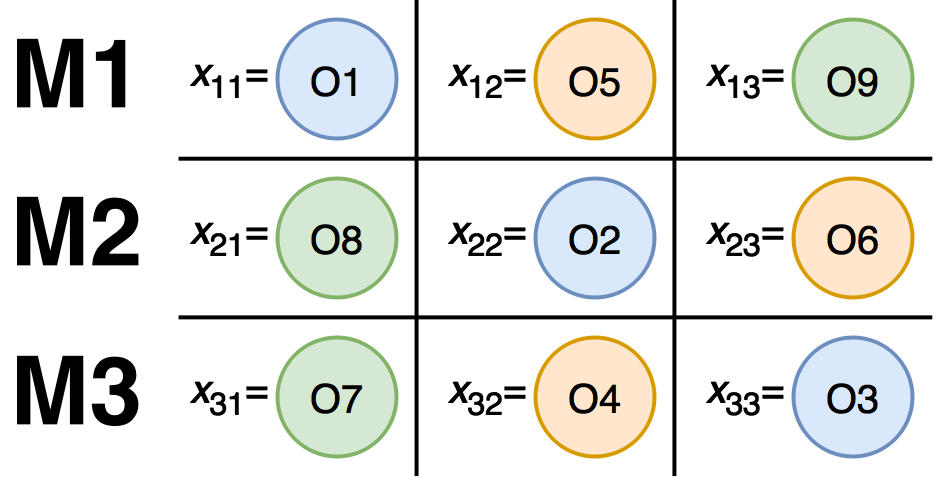
\includegraphics[scale=0.2]{figures/permve-ntnu-it3708-project-4-2017-schedule-representation}
\captionof{figure}{A \acs{JSSP} schedule is represented as an $m \times n$ matrix of $m$ machines and $n$ jobs. \textcolor{NavyBlue}{$\text{Job~1} = \langle\,\text{O}_1, \text{O}_2, \text{O}_3\,\rangle$}, \textcolor{Melon}{$\text{Job~2} = \langle\,\text{O}_4, \text{O}_5, \text{O}_6\rangle$}, \textcolor{OliveGreen}{$\text{Job~3} = \langle \text{O}_7, \text{O}_8, \text{O}_9\rangle$}. Each row $i$ encodes the ordering of operations for machine $i$; $M_1, M_2, M_3$.}
\label{figure:representation}
\vspace{0.3cm}
}

\section*{\acl{PSO}}

\acf{PSO} is an optimization technique mostly applied to problems with continuous solution spaces, where each particle in a swarm represents a solution. To solve a discrete problem such as \ac{JSSP}, inspiration has been taken from \cite{sha2006hybrid}. The resulting algorithm uses a discrete, preference-based representation, a modified approach velocity update, a modified approach to position updates, a diversification strategy, and a local search. The overall algorithm can be described by the following three steps:

\begin{enumerate}
    \item The initial swarm population is generated, where the position of each particle $k$ is represented by a matrix of preferred machine operations $x^k$ as shown in Figure~\ref{figure:representation}. The job ordering for each machine is shuffled randomly, before the position of each particle $x^k$ is developed by the G\&T algorithm into a feasible schedule $S^k$.
    \item For each solution $S^k$ represented by particle $k$ in the swarm, its best historical schedule, as determined by the schedule makespan, is tracked as $\textit{pbest}^k$. The best solution out of all particles is tracked as \textit{gbest}.
    \item If the maximum number of iterations has not been reached:
    \begin{enumerate}
        \item Update the velocity $v^k$ for each particle $k$.
        \item For each particle $k$ in the swarm; update its position $x^k$ and develop the position $x^k$ into the schedule $S^k$. For each schedule $S^k$, apply \ac{TS}, before updating $\textit{pbest}^k$ and \textit{gbest} accordingly.
    \end{enumerate}
\end{enumerate}

The velocity of each particle $k$ is represented by an $m \times n$ matrix, where the velocity of each operation $o_{ij}$ is denoted by $v_{ij} \in \{0,1\}$, and $o_{ij}$ is the operation of job~$j$ on machine~$i$. When $v_{ij}^k = 1$, the operation $o_{ij}$ of particle $k$ has just been moved to its current position in $x^k$, and cannot be moved. In this way, the adapted velocity mechanism imitates the behavior of continuous velocity by providing the discrete representation with momentum. The velocity $v_{ij}^k$ is randomly set to zero with a probability $(1-w)$ when updating the velocity of each particle.

{
\vspace{0.2cm}
\begin{minipage}{\linewidth{}}
\centering
\begin{tabular}{lc}
\toprule
Parameter                                   & Value \\
\midrule
Iterations                                  & 150   \\
Swarm size                                  & 100   \\
Particle best factor ($c_1$)                &   0.5 \\
Global best factor ($c_2$)                  &   0.3 \\
Probability of not resetting velocity ($w$) &   0.5 \\
\bottomrule
\end{tabular}
\vspace{-0.2cm}
\captionof{table}{\acf{PSO} parameters.}
\label{table:psoparams}
\end{minipage}
}

Position updates relate to the discrete velocities. If $v_{ij}^k=0$, the operation $o_{ij}^k$ will be moved to the corresponding location of operation $o_{ij}^k$ in $\textit{pbest}^k$ with probability $c_1$, or it will be moved to the corresponding location of $o_{ij}^k$ in \textit{gbest} with probability $c_2$. In this manner, the $\textit{pbest}$ and \textit{gbest} solutions are used to guide the global \ac{PSO} search. The position update is performed as follows for each machine $i$:

\begin{enumerate}
    \item Randomly select a location $l$ in $x_i^k$.
    \item Denote the operation at location $l$ in $x_i^k$ by $O_1$.
    \item Find the location of operation $O_1$ in $\textit{pbest}_i^k$ with probability $c_1$, or find the location of operation $O_1$ in $\textit{gbest}_i$ with probability $c_2$. Denote the location found in $\textit{pbest}_i^k$ or $\textit{gbest}_i$ by $l'$, and denote the operation at location $l'$ in $x_i^k$ by $O_2$.
    \item If $O_2$ has been denoted, and the velocity components $v_{i{J_1}}^k$ and $v_{i{J_2}}^k$ for jobs $J_1$ and $J_2$, associated with operations $O_1$ and $O_2$, are both zero, then swap operations $O_1$ and $O_2$ in $x_i^k$, and set $v_{i{J_1}}^k \gets 1$.
    \item If all locations in $x_i^k$ has been considered, then the velocity update is completed. Otherwise, if $l<n$, set $l \gets l+1$, else assign $l \gets 1$, and continue from step~2.
\end{enumerate}

To prevent the \ac{PSO} search from getting stuck in local minima, a diversification strategy is used when updating $\textit{pbest}^k$ and \textit{gbest}. For each new solution $S^k$, the following update is used:

\begin{enumerate}
    \item If the makespan of $S^k$ is less than the makespan of \textit{gbest}, set the $\textit{pbest}$ solution with the worst makespan to the current \textit{gbest}, and set \textit{gbest} to $S^k$.
    \item Otherwise, if the makespan of $S^k$ is equal to the makespan of any $\textit{pbest}$ or the \textit{gbest} solution, replace the solution with the equal makespan with $S^k$.
    \item Otherwise, if the makespan of $S^k$ is better than the makespan of the worst $\textit{pbest}$ solution, set the worst $\textit{pbest}$ solution to $S^k$.
\end{enumerate}

The implemented \ac{PSO} uses Taboo search as described in \cite{nowicki1996fast} with backtracking and cycle detection. This local search, using parameters shown in Table~\ref{table:tsparams}, assists the global \ac{PSO} search, which uses parameters shown in Table~\ref{table:psoparams}. The mutation operation described in \cite{sha2006hybrid} is not used.

\section*{\acl{ACO}}

\acf{ACO} is a swarm search inspired by how ants are able to locate food and direct other ants towards discovered food sources by using pheromones. The pheromone information is a central component in \ac{ACO} by guiding the search through learning the relations between related operations as described in \cite{blum2004ant}. An operation $o_a$ is related to an operation $o_b$ if they are directly adjacent in a job sequence, or if they have to be processed by the same machine. The set of operations related to operation $o_a$ is denoted by $\mathcal{R}_a$.

The pheromone information is represented as an $\vert O \vert \times \vert O \vert$ matrix $\mathcal{T}$, where an entry $\mathcal{T}_{ab}$ represents the desirability of processing operation $o_a$ before operation $o_b$ with a specific value denoted by $\tau_{ab}$. Solutions are generated from the pheromone information using an algorithm similar to G\&T, with the exception of how the conflict set $C$ is chosen in step~3a, and how an operation is selected from $C$ in step~3b. This process will always generated feasible schedules.

In 50\% of cases, the conflict set is set to produce non-delay schedules; $C = \{o \in \Omega \vert s_o = \min_{o' \in \Omega} s_{o'}\}$. In the other cases, the conflict set is not limiting; $C = \Omega$.

The selection of an operation from the conflict set $C$ is done by drawing randomly according to the probabilities:

\begin{equation}
p(o_a \vert \mathcal{T}) = \frac
{
    \min_{o_b \in \mathcal{R}_a \cap O^{+}} \tau_{ab} \cdot \eta(o_a)^\beta
}
{
    \sum_{o_c \in C} \min_{o_b \in \mathcal{R}_a \cap O^{+}} \tau_{ab} \cdot \eta(o_a)^\beta
}, \quad \forall o_a \in C
\label{eq:acopoa}
\end{equation}

Where $O^{+}$ is the set of operations which has not yet been added to the schedule, and $\eta(o_a)$ is the heuristic information given by:

\begin{equation}
\eta(o_a) = \frac
{
    \frac{1}{s_{o_a} + 1}
}
{
    \sum_{o_c \in C} \frac{1}{s_{o_a} + 1}
}
\label{eq:acoheur}
\end{equation}

The \ac{ACO} search can be described by the following four steps, which are repeated for as long as necessary:

\begin{enumerate}
    \item Generate $n_a = \max \Big\{ 10, \big\lfloor \frac{\vert O \vert}{10} \big\rfloor \Big\}$ solutions to form the generation $\mathcal{G}$, using the G\&T algorithm with modified conflict set (Equation~\ref{eq:acopoa}) and selection (Equation~\ref{eq:acoheur}), where $n_a$ is the number of ants.
    \item Apply local search to improve each schedule in $\mathcal{G}$.
    \item Apply \ac{TS} to the schedule with the lowest makespan in $\mathcal{G}$.
    \item Update the pheromones according to Equation~\ref{eq:acophero}~and~\ref{eq:acodelta}, where $\eta$ is the rate of pheromone evaporation, and $S^{*}$ is the best schedule found by the \ac{ACO} search.
\end{enumerate}

\begin{equation}
\tau_{ab} \gets \tau_{ab} + \rho \cdot \big[ \delta(o_a, o_b) - \tau_{ab} \big]
\label{eq:acophero}
\end{equation}

\begin{equation}
\delta(o_a, o_b) =
\begin{cases}
1, \text{if $o_a$ is processed before $o_b$ in $S^{*}$}\\
0, \text{otherwise}
\end{cases}
\label{eq:acodelta}
\end{equation}

Pheromone values are limited to the range $[0.001, 0.999]$.

{
\vspace{0.2cm}
\begin{minipage}{\linewidth{}}
\centering
\begin{tabular}{lc}
\toprule
Parameter                                         & Value \\
\midrule
Iterations                                        & 20    \\
Heuristic power ($\beta$)                         & 10.0  \\
Evaporation rate ($\rho$)                         &  0.1  \\
Initial pheromone value ($\tau_{\text{initial}}$) &  0.5  \\
\bottomrule
\end{tabular}
\vspace{-0.2cm}
\captionof{table}{\acf{ACO} parameters.}
\label{table:acoparams}
\end{minipage}
}

\section*{\acl{BA}}

\acf{BA} is a swarm search inspired by how bees locate and coordinate the gathering of food \cite{pham2011bees}. The implemented version of the algorithm for the \ac{JSSP} problem can be described in 2 steps:

\begin{enumerate}
    \item A number $n$ of preference matrices are generated as shown in Figure~\ref{figure:representation}, where the job ordering for each machine is shuffled, before each preference matrix is developed by the G\&T algorithm into a schedule description. These $n$ solutions represent the sites located by the $n$ scouting bees.
    \item While the search is not complete:
    \begin{enumerate}
        \item For each of the best $e$ sites out of $n$, as determined by makespan, deploy $nep$ bees. These bees each represent a \ac{TS} search from the elite site. For each of the elite sites, the best solution out of $nep$ solutions is used as a site in the next generation.
        \item For each of the following best $(m-e)$ sites out of $n$, as determined by makespan, deploy $nsp$ bees. These bees each represent a local search from the normal site. For each of the normal sites, the best solution out of $nsp$ is used as a site in the next generation.
        \item Any remaining $(n-m)$ scouting bees are used to locate new solutions which are generated in the same way as the initial sites in step~1 and used as sites in the next generation.
    \end{enumerate}
\end{enumerate}

The original version of the algorithm \cite{pham2011bees} is used on continuous optimization problems, and the searching behavior for the elite and normal sites are the same, with the exception that more bees are used to search elite sites compared to normal sites. In the adapted version of the algorithm for the \ac{JSSP}, a stronger local search is instead used to strengthen the search for elite sites, by employing a full \ac{TS} for elite sites, and a simpler local search for normal sites.

{
\vspace{0.2cm}
\begin{minipage}{\linewidth{}}
\centering
\begin{tabular}{lc}
\toprule
Parameter                              & Value \\
\midrule
Iterations                             &  5 \\
Number of scouts ($n$)                 & 10 \\
Number of sites selected ($m$)         &  8 \\
Number of elite sites ($e$)            &  3 \\
Number of normal sites ($m-e$)         &  5 \\
Number of bees per elite site ($nep$)  &  1 \\
Number of bees per normal site ($nsp$) &  2 \\
\bottomrule
\end{tabular}
\vspace{-0.2cm}
\captionof{table}{\acf{BA} parameters.}
\label{table:baparams}
\end{minipage}
}

\section*{\acl{TS}}

Several papers \cite{sha2006hybrid}\cite{blum2004ant} on the \ac{JSSP} reference the \ac{TS} detailed in \cite{nowicki1996fast}. This search is based on searching the neighborhood $H(S)$ of a schedule, which is established by the set of all moves deemed ``interchanges near the borderline of blocks on a single critical path''. Given a schedule, any longest sequence of operations in the schedule is called a critical path. An arbitrary selected critical path of $S$ is considered. For this path, blocks of operations $B_1, \ldots, B_r$ which share a machine is considered. The set of considered swapping moves $V(S)$ is defined as all moves which swap the last two operations in the first block, the first or last two operations in any middle block, or the first two operations in the last block. The neighborhood of $S$ is then $H(S) = \{ Q(S, v) : v \in V(S)\}$, where $Q(S, v)$ is the schedule resulting from applying move $v$ to $S$.

{
\vspace{0.3cm}
\centering
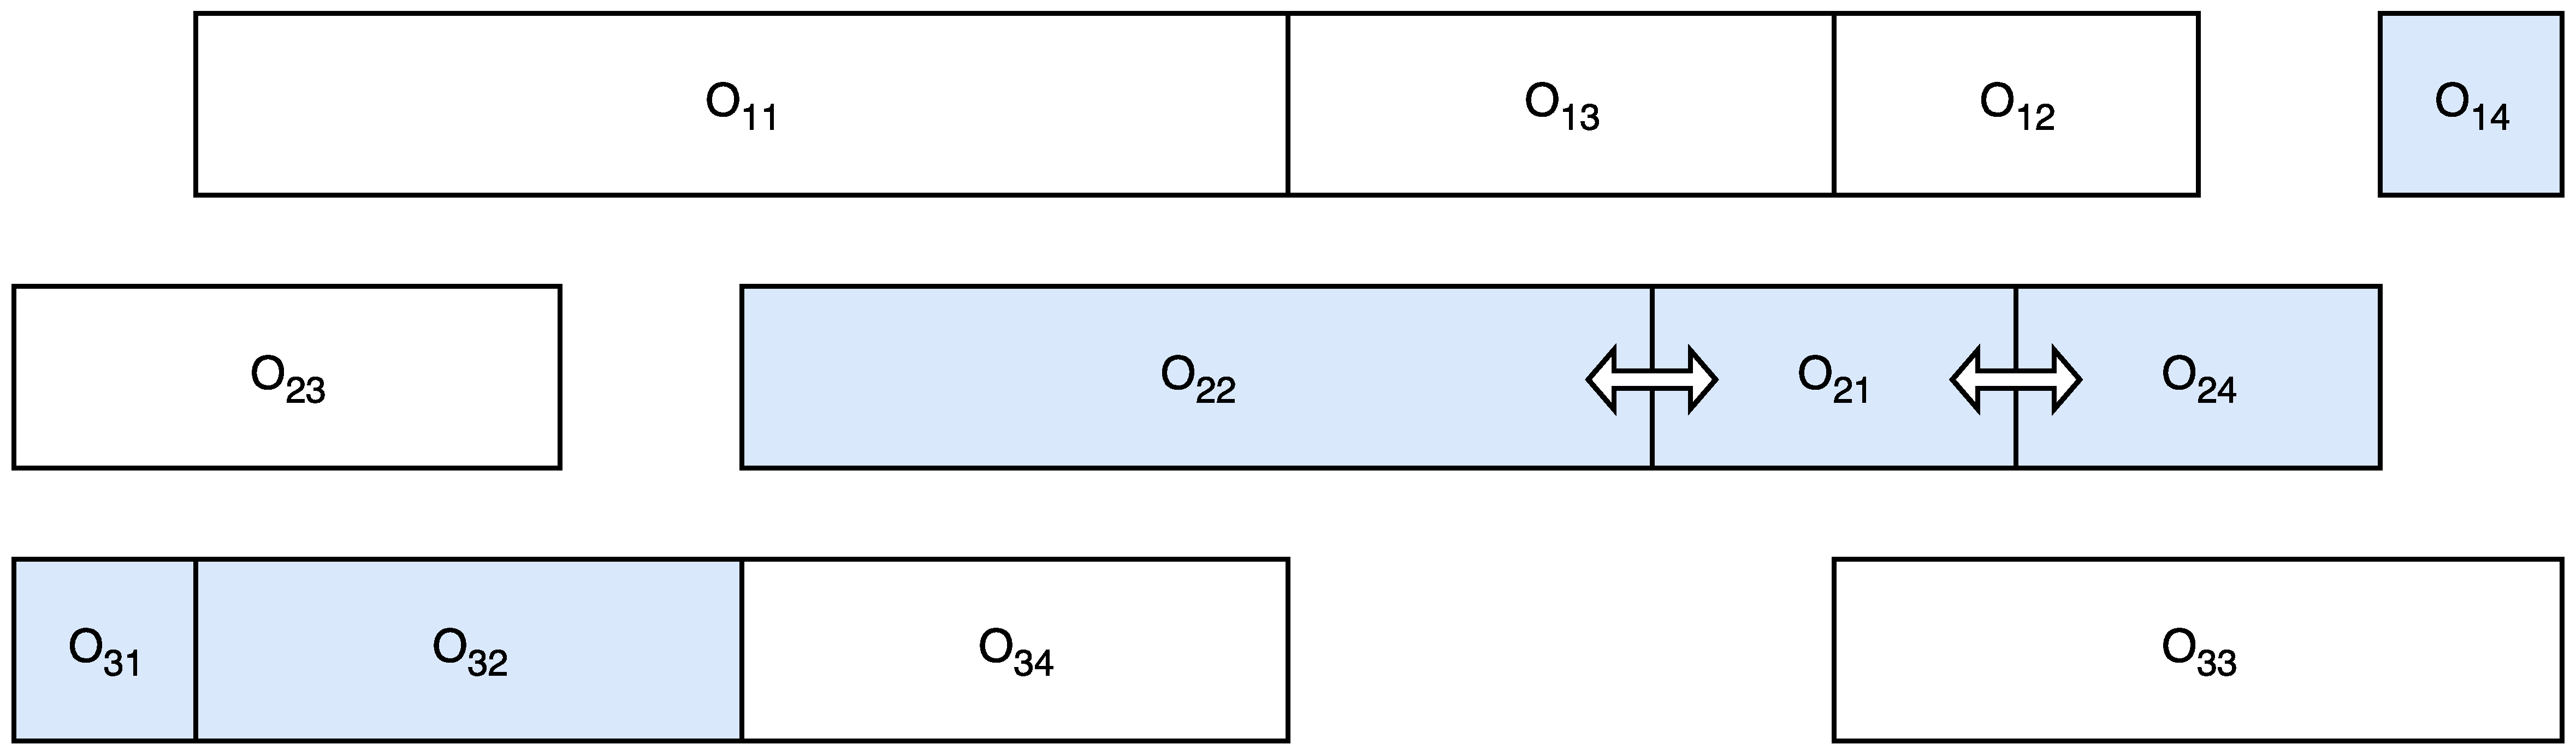
\includegraphics[scale=0.1]{figures/permve-ntnu-it3708-project-4-2017-neighborhood}
\captionof{figure}{An example showing the critical path in shaded blue, and the set of possible swaps defined by $V(S)$.}
\label{figure:neighborhood}
\vspace{0.3cm}
}

Central to the \ac{TS} is the \ac{NSP} which takes a schedule $S$, a set of moves $V$, a taboo list $T$ of forbidden moves, and the best makespan found; $C^*$. The taboo list is a queue with maximum size \textit{maxt}. The procedure returns a selected $v'$ and the schedule $S'$ which is the result of applying $v'$ to $S$. It can be described in three steps:

\begin{enumerate}
    \item Find the set of moves $A$ which are forbidden by the taboo list, but which are ``profitable'', i.e. the moves which lead to a schedule $S'$ with a lower makespan than $C^*$:
    \begin{equation}
        A = \{v \in V(S) \cap T : C_{\max}(Q(S, v)) < C^*\},
    \end{equation}
    where $C_{\max}(S)$ denotes the makespan of schedule $S$. If $(V(S) \setminus T) \cup A \ne \varnothing$, i.e. if there are any unforbidden moves or any profitable forbidden moves, then select a move $v'$ such that:
    \begin{equation}
        \small
        C_{\max}(Q(S, v')) = \min \{ C_{\max}(Q(S, v)) : v \in (V(S)\setminus T) \cup A \},
    \end{equation}
    and continue from step 3.
    \item If $|V(S)|=1$, then select $v' \in V(S)$. Otherwise, append the last move in the taboo list to the taboo list until ${ V(S)\setminus T \ne \varnothing }$. Then select ${v' \in V(S)\setminus T}$.
    \item Set $S' \gets Q(S, v')$ and append $v'$ to $T$.
\end{enumerate}

In the case of the \ac{PSO} and \ac{BA} implementations, the local search used is to simply apply a single randomly selected move $v'$ from the neighborhood $H(S)$ of a schedule, without a taboo list. In addition to using the same local search in the case of \ac{ACO}, a full \ac{TS} is also used to improve the best solution in each iteration. The \acl{TS} consists of applying the \acl{NSP} repeatedly to a schedule for a number of iterations, while keeping track of the best schedule and makespan found. Backtracking and cycle detection was also implemented as part of the \ac{TS} as described in \cite{nowicki1996fast}.

{
\vspace{0.5cm}
\begin{minipage}{\linewidth{}}
\centering
\begin{tabular}{lc}
\toprule
Parameter                                                 & Value \\
\midrule
Iteration limit (\textit{maxiter})                        &   150 \\
Total iteration limit ($\textit{maxiter}_\textit{total}$) &  1000 \\
Taboo list limit (\textit{maxt})                          &     5 \\
Backtracking limit (\textit{maxl})                        &     8 \\
Max cycle detection count ($\max c$)                      &     2 \\
Max cycle detection duration ($\max \delta$)              &   100 \\
\bottomrule
\end{tabular}
\vspace{-0.2cm}
\captionof{table}{\acf{TS} parameters.}
\label{table:tsparams}
\end{minipage}
}

\bibliographystyle{unsrt}
\bibliography{references.bib}

\end{multicols}

% For test problem #3, draw the gantt-chart targeting the best makespan. You need to draw for all three algorithms. (1.5p)

\begin{landscape}
{
\begin{table}
\hspace*{-0.5cm}
\centering
\begin{tabular}{l}
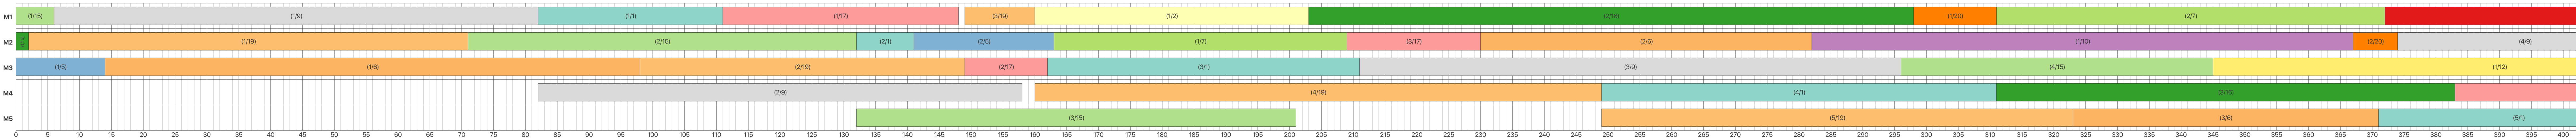
\includegraphics[height=40pt]{figures/solution_pso_instance_3_1_scaled}\\[0.15cm]
\hspace{0.90909pt}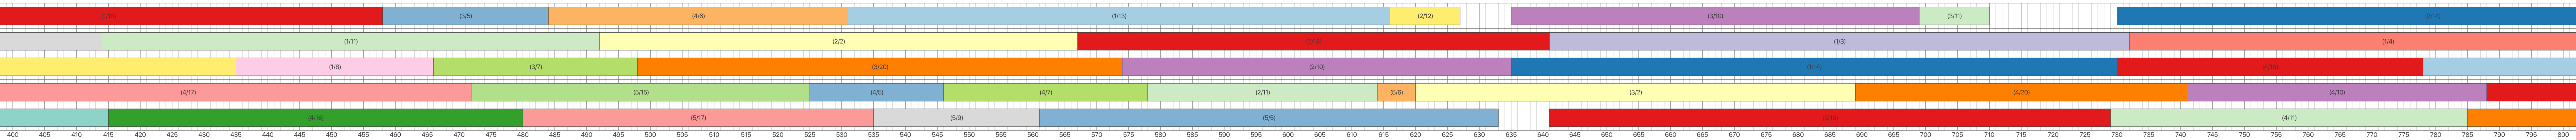
\includegraphics[height=40pt]{figures/solution_pso_instance_3_2_scaled}\\[0.15cm]
\hspace{0.90909pt}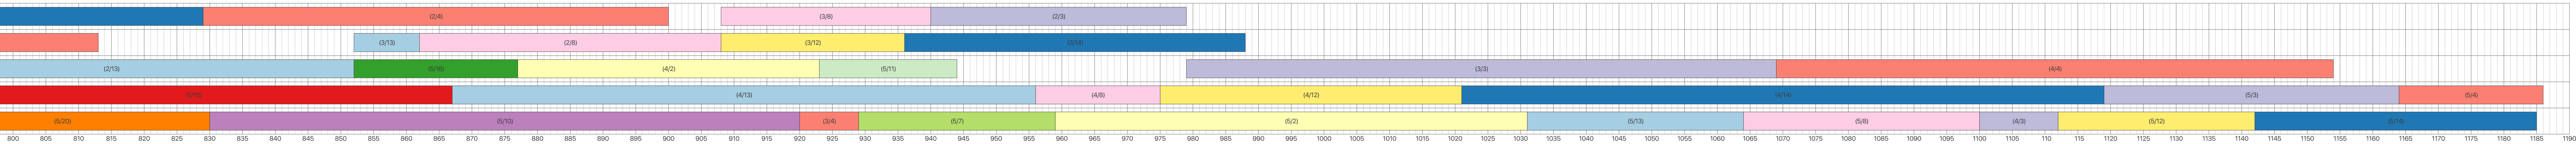
\includegraphics[height=40pt]{figures/solution_pso_instance_3_3_scaled}\\
\multicolumn{1}{c}{\textit{Figure 1: \acf{PSO} solution with makespan 1186 for problem~3 using parameters specified in Table~\ref{table:psoparams}~and~\ref{table:tsparams}.}}\\[1.2cm]
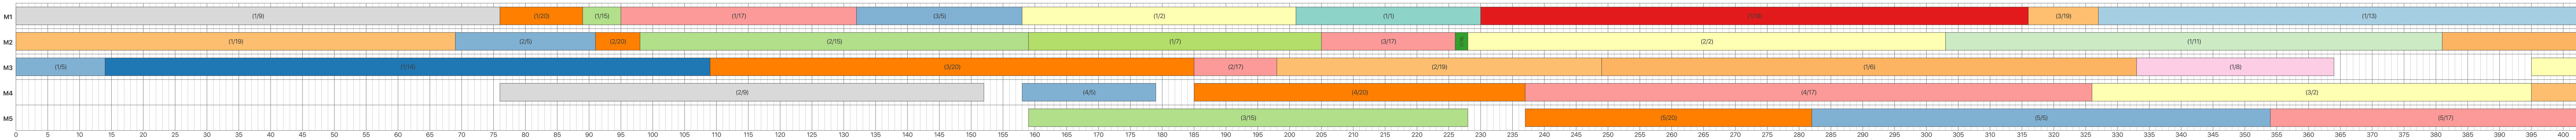
\includegraphics[height=40pt]{figures/solution_aco_instance_3_1_scaled}\\[0.15cm]
\hspace{0.90909pt}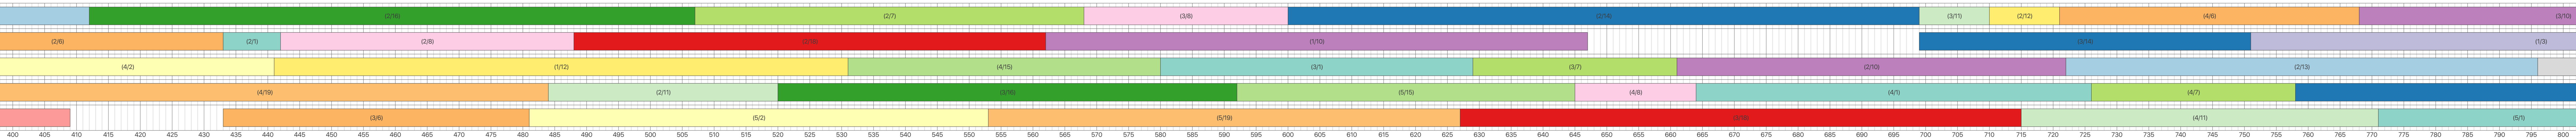
\includegraphics[height=40pt]{figures/solution_aco_instance_3_2_scaled}\\[0.15cm]
\hspace{0.90909pt}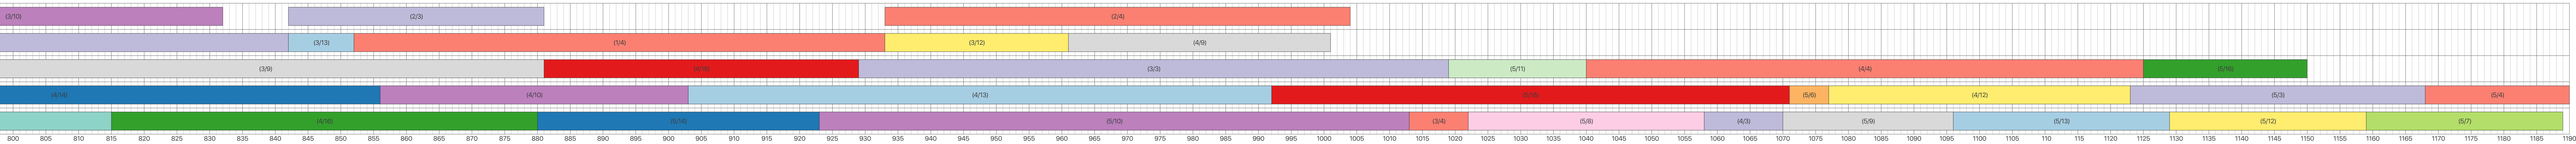
\includegraphics[height=40pt]{figures/solution_aco_instance_3_3_scaled}\\
\multicolumn{1}{c}{\textit{Figure 2: \acf{ACO} solution with makespan 1190 for problem~3 using parameters specified in Table~\ref{table:acoparams}~and~\ref{table:tsparams}.}}\\[1.2cm]
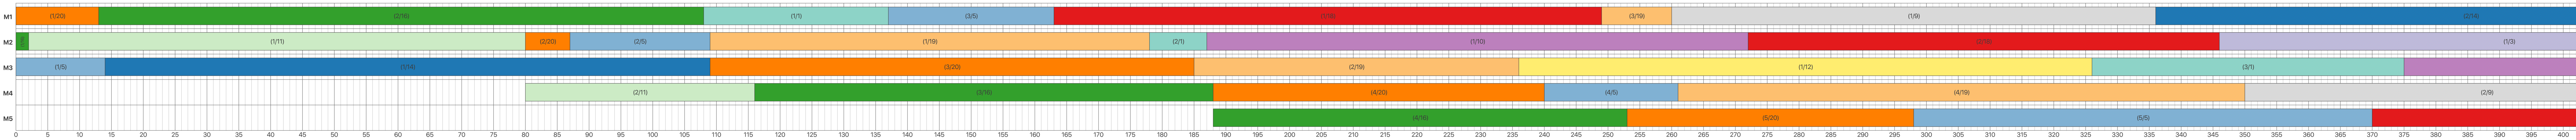
\includegraphics[height=40pt]{figures/solution_ba_instance_3_1_scaled}\\[0.15cm]
\hspace{0.90909pt}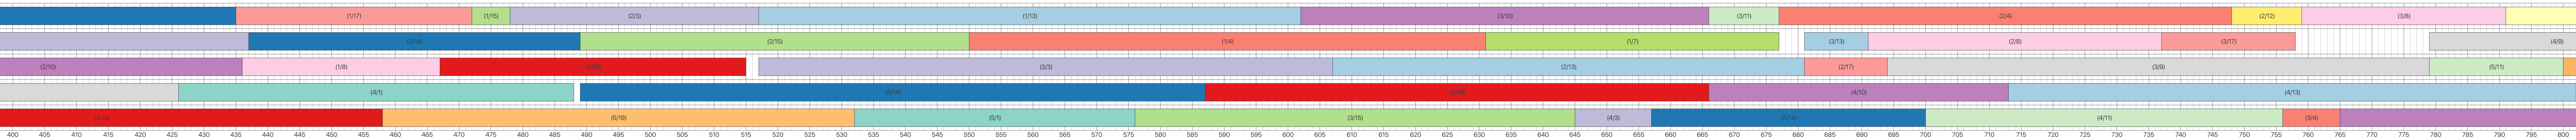
\includegraphics[height=40pt]{figures/solution_ba_instance_3_2_scaled}\\[0.15cm]
\hspace{0.90909pt}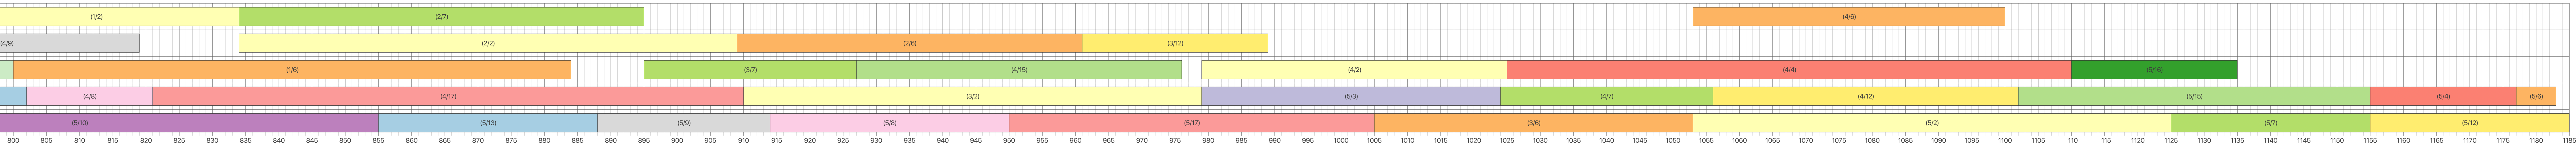
\includegraphics[height=40pt]{figures/solution_ba_instance_3_3_scaled}\\
\multicolumn{1}{c}{\textit{Figure 3: \acf{BA} solution with makespan 1185 for problem~3 using parameters specified in Table~\ref{table:baparams}~and~\ref{table:tsparams}.}}\\
\end{tabular}
\end{table}
}
\end{landscape}

\end{document}
